\documentclass{article}
\usepackage{graphicx} % Required for inserting images
\title{Progress Documentation}
\author{Ali Ali}
\date{September 2025}
\graphicspath{ {./imgs/} }

\begin{document}
\maketitle
\begin{figure}
  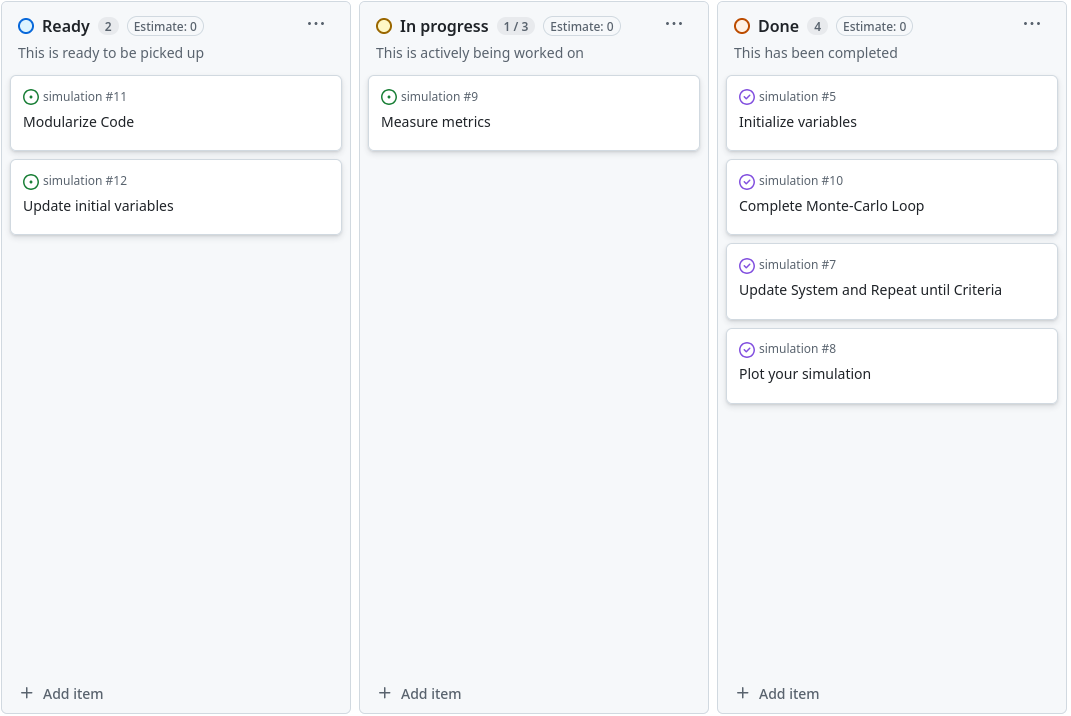
\includegraphics[scale=0.4]{projectboard}
  \caption{Project Board}
\end{figure}

\begin{figure}
  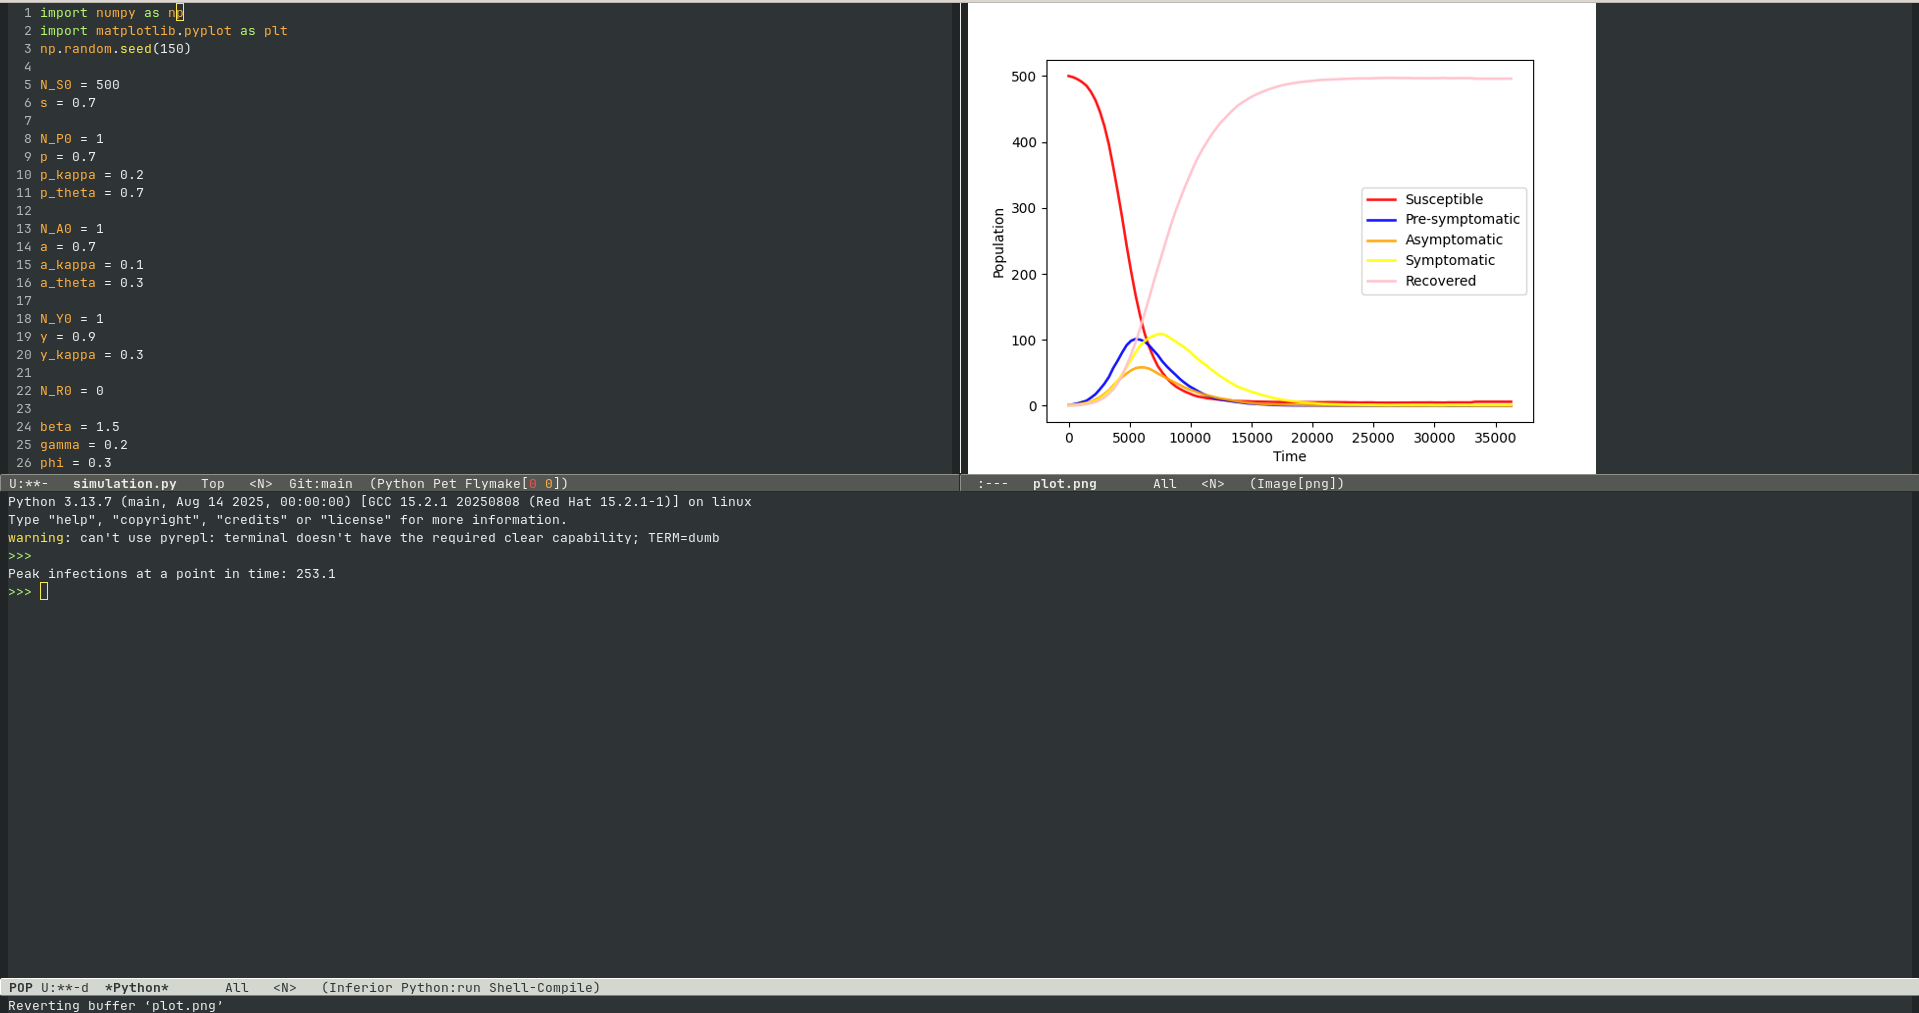
\includegraphics[scale=0.3]{running1.png}
  \caption{A simulation run with the inputs (top left) outputting metrics (bottom) and graph showing the change in each compartment over time (top right).}
\end{figure}
\begin{figure}
  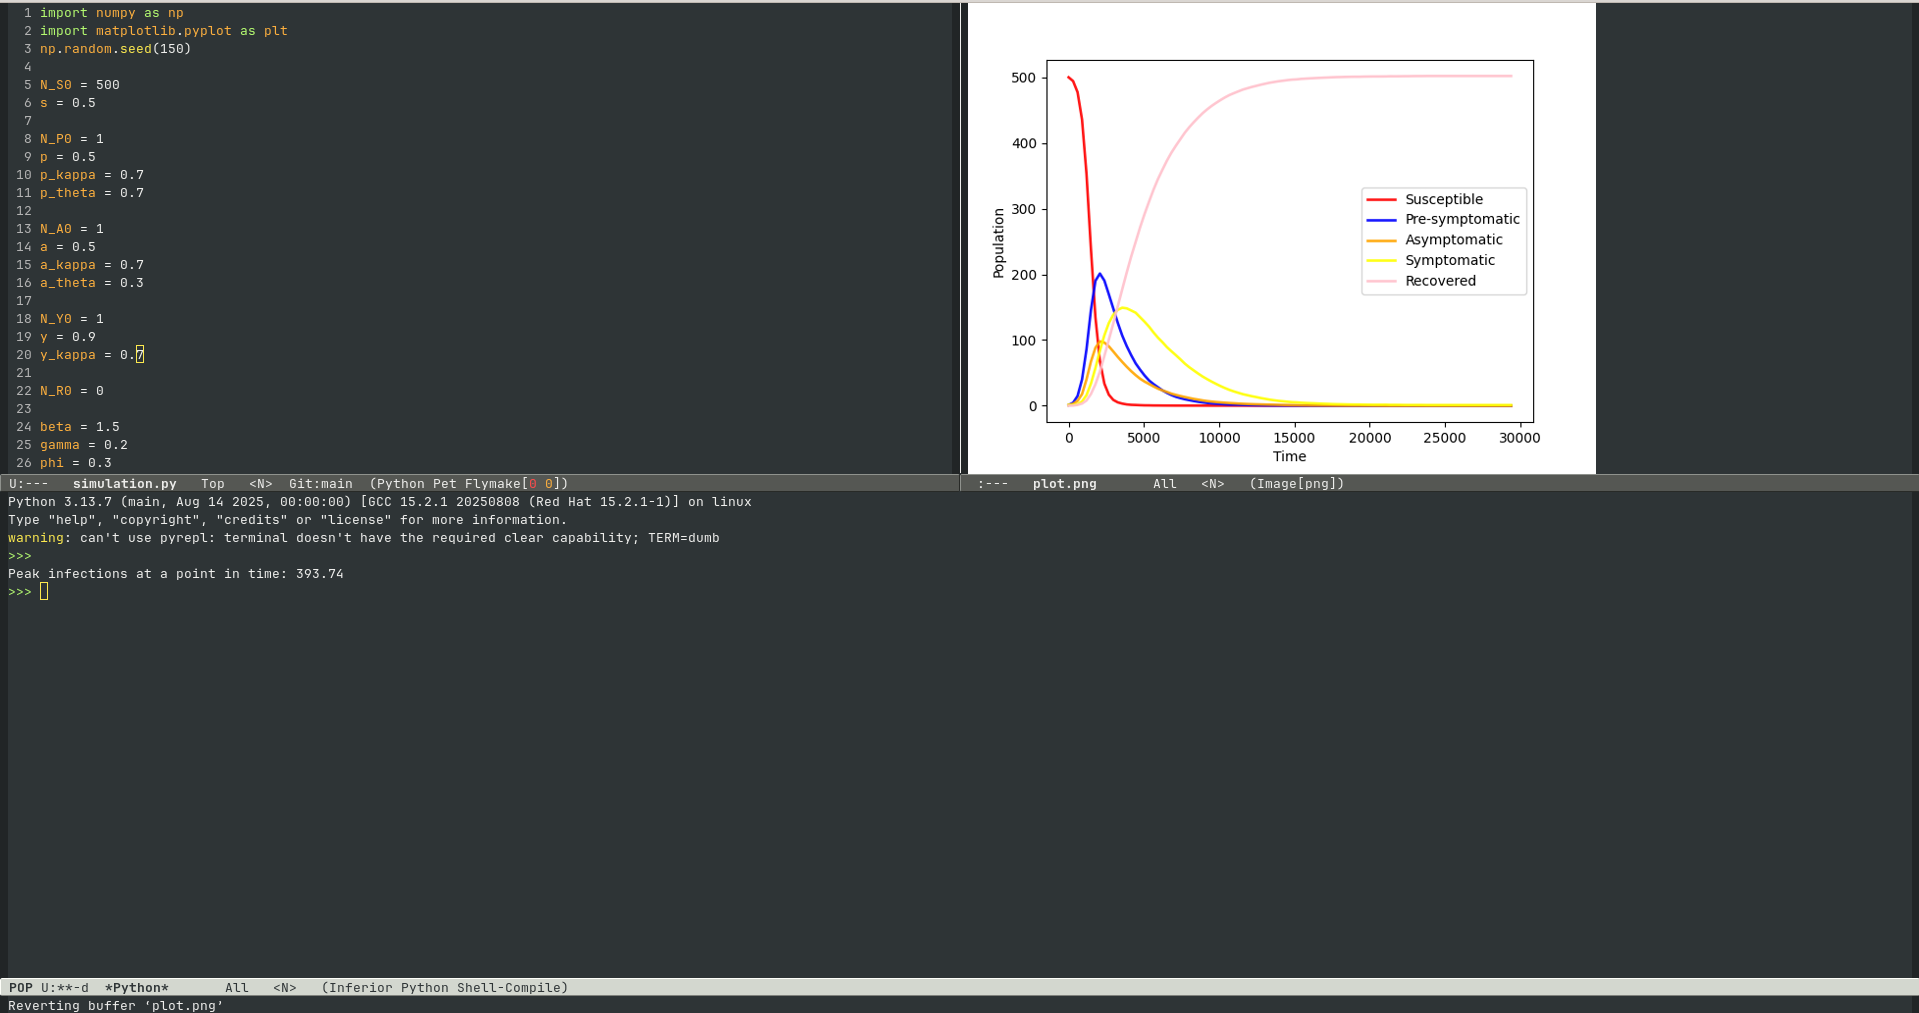
\includegraphics[scale=0.3]{running2.png}
  \caption{A simulation run with the inputs (top left) outputting metrics (bottom) and graph showing the change in each compartment over time (top right).}
\end{figure}
\begin{figure}
  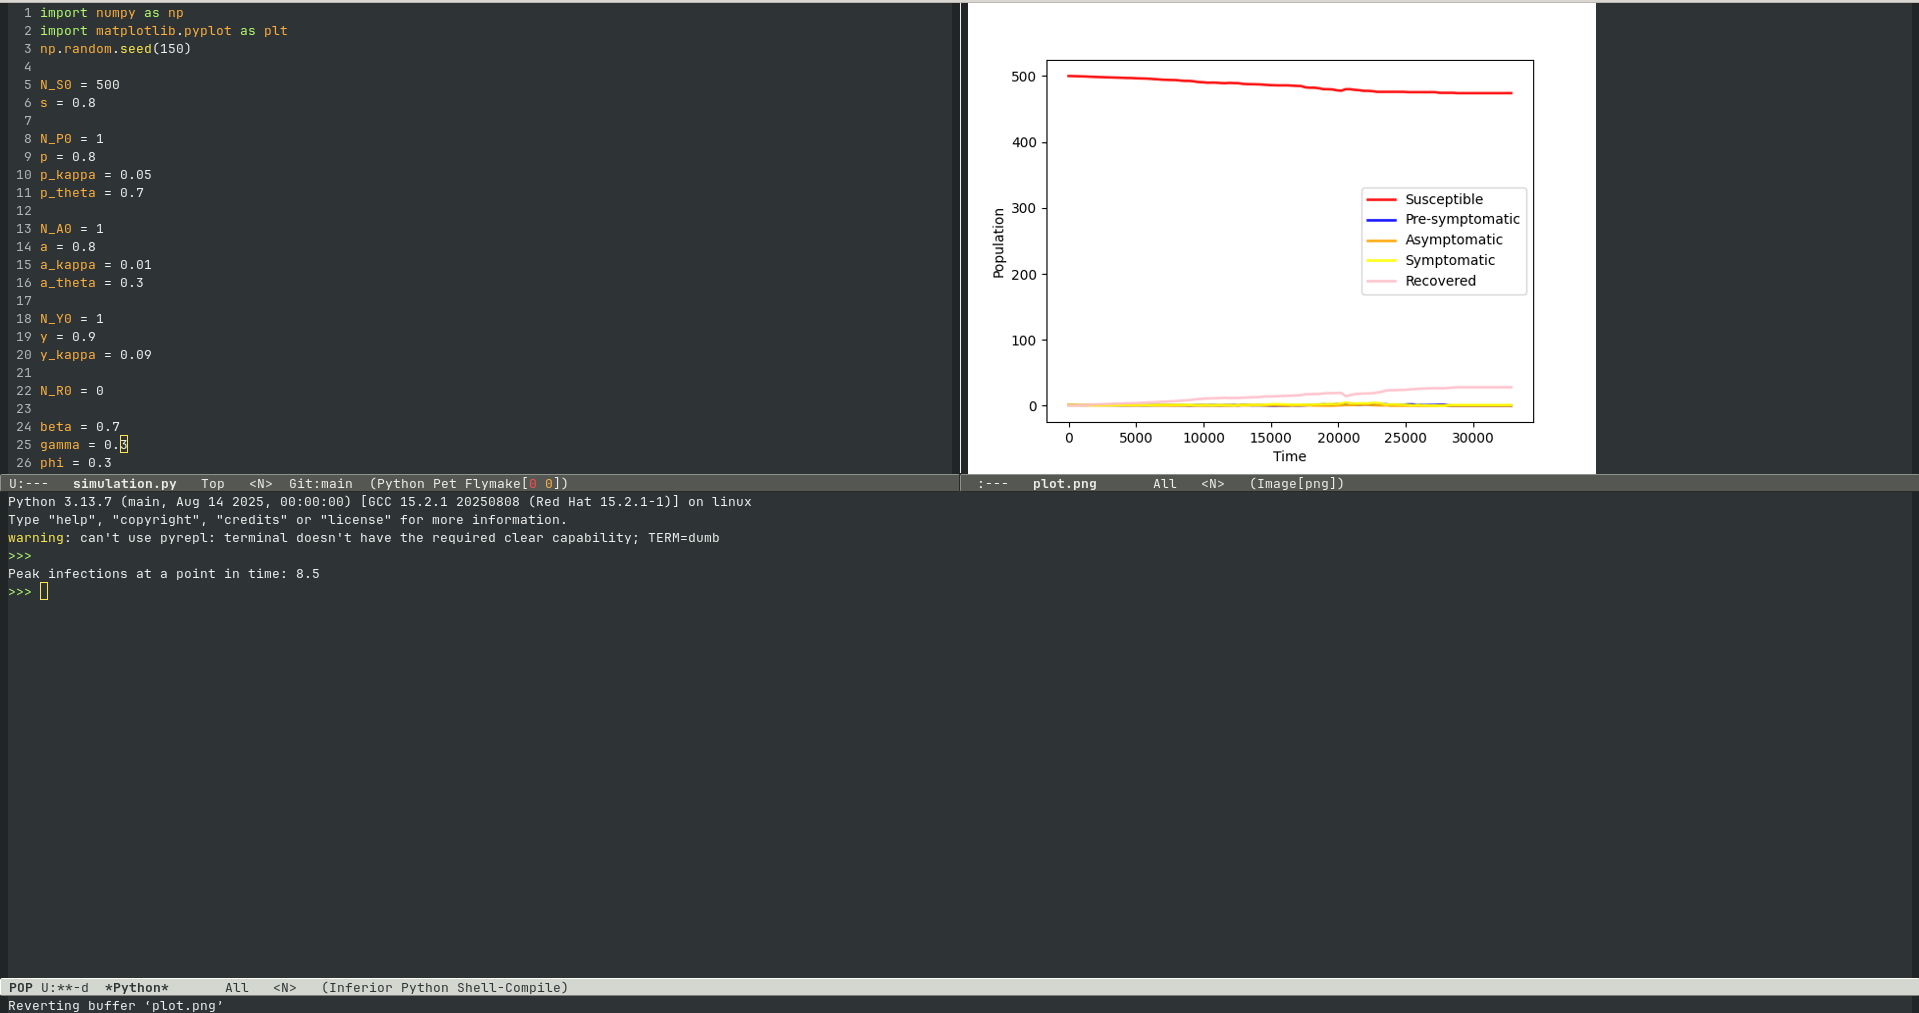
\includegraphics[scale=0.3]{running3.png}
  \caption{A simulation run with the inputs (top left) outputting metrics (bottom) and graph showing the change in each compartment over time (top right).}
\end{figure}
\begin{figure}
  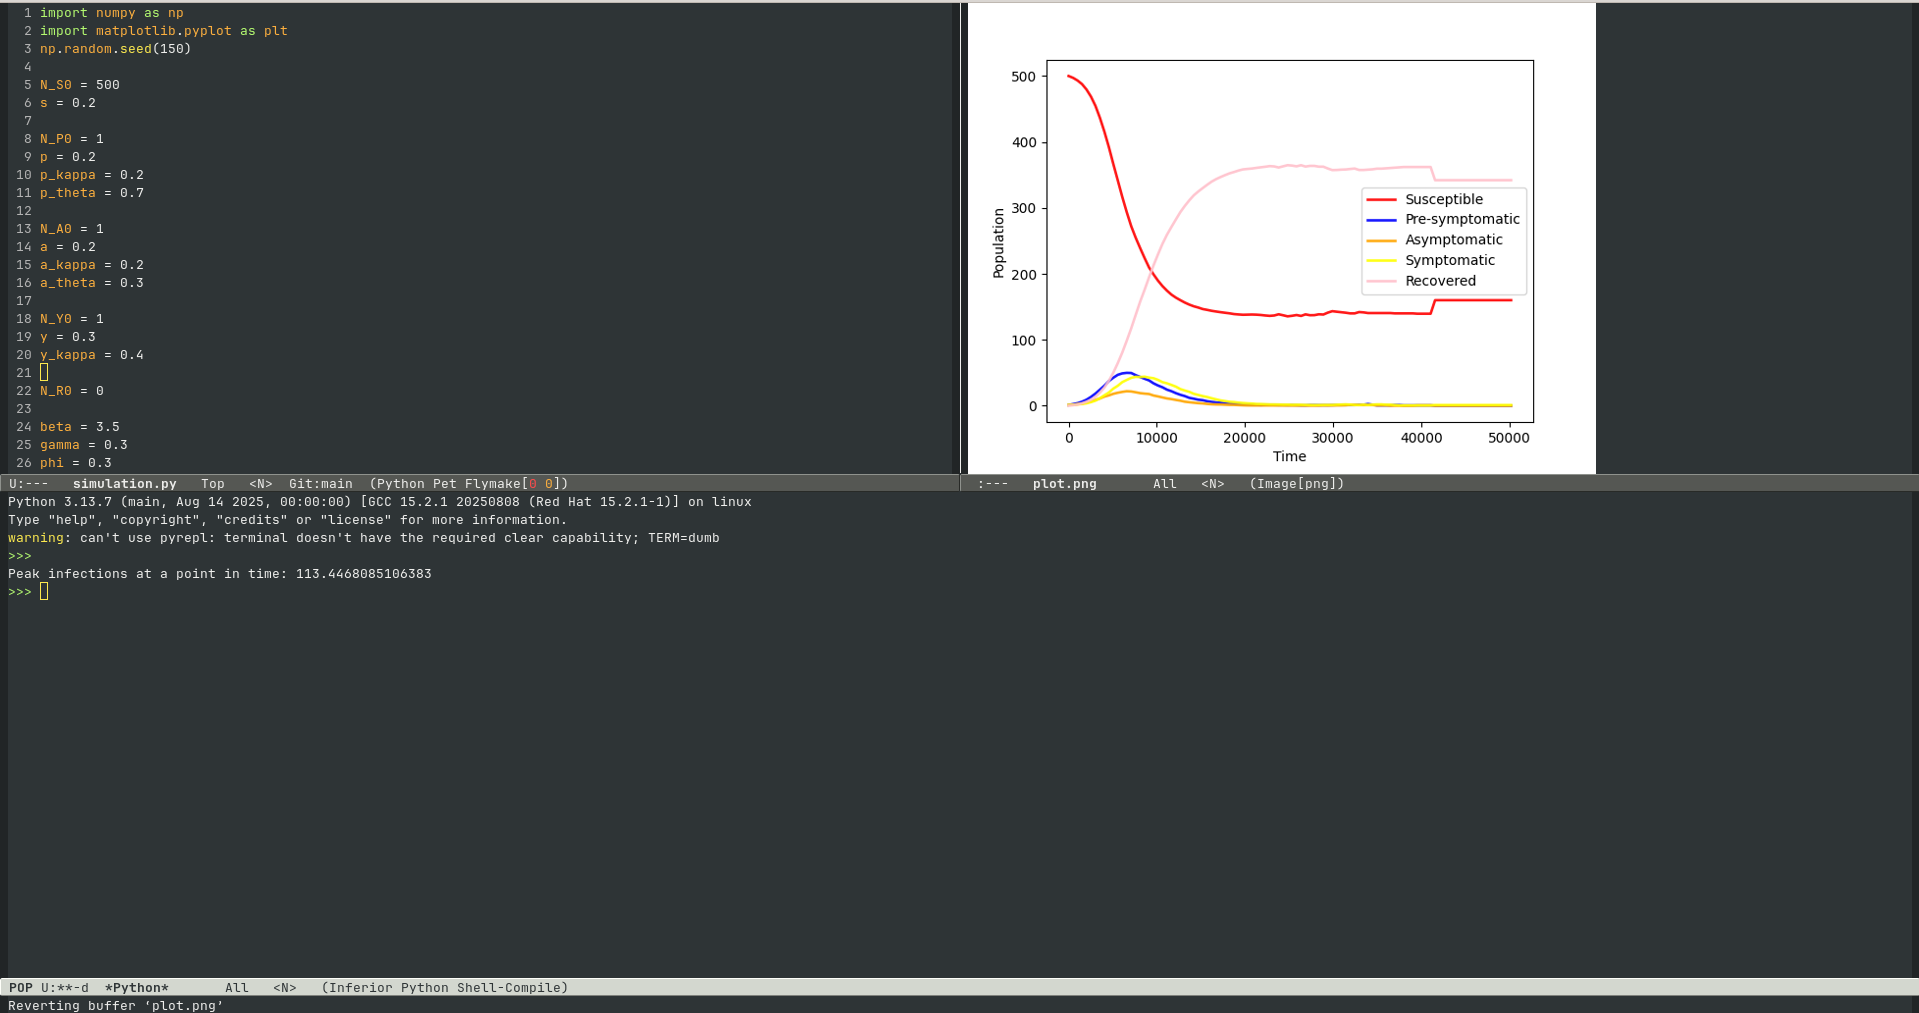
\includegraphics[scale=0.3]{running4.png}
  \caption{A simulation run with the inputs (top left) outputting metrics (bottom) and graph showing the change in each compartment over time (top right).}
\end{figure}

Currently, the initial variables, the main simulation loop, a result plot, and the peak infections at a point in time metric have been completed. What has not been completed is choosing real-world values for the initial variables, the rest of the metrics, and modularizing the code. Our key accomplishment is the main simulation loop which is a Monte-Carlo loop that randomly simulates the time until next event following a Poisson process and chooses an event according to a probability distribution. A key challenge faced was determining how to choose the event according to its probability which was solved by dividing each probability by the total event rate, to ensure the probability distribution adds up to a 100, and then using the numpy.random.choice function.


\end{document}
